\documentclass{article}
\usepackage{graphicx}
\usepackage{amsmath}
\usepackage{pgfplots}
\usepackage{array}
\usepackage[margin=1.5cm]{geometry}
\usepackage{adjustbox}
\usepackage{hyperref}
\usepackage{cite}
\usepackage{listings}
\usepackage{xcolor}
\usepackage{comment}
\usepackage{graphicx}
\usepackage{pdfpages}
\usepackage{enumitem}
\usepackage{pgfplotstable}
\usepackage{booktabs}
\usepackage{adjustbox}
\usepackage{changepage}
\usepackage[utf8]{inputenc}
\lstset{ 
literate= {á}{{\'a}}1 
    {é}{{\'e}}1 
    {í}{{\'i}}1 
    {ó}{{\'o}}1 
    {ú}{{\'u}}1
} 

\hypersetup{
colorlinks=true,
linkcolor=blue,
urlcolor=blue,
}

\pgfplotsset{compat=1.17}
\usepackage[portuguese]{babel}

\definecolor{codegreen}{rgb}{0,0.6,0}
\definecolor{codegray}{rgb}{0.5,0.5,0.5}
\definecolor{codepurple}{rgb}{0.58,0,0.82}
\definecolor{backcolour}{rgb}{0.95,0.95,0.92}

\lstdefinestyle{mystyle}{
    backgroundcolor=\color{backcolour},   
    commentstyle=\color{codegreen},
    keywordstyle=\color{magenta},
    numberstyle=\tiny\color{codegray},
    stringstyle=\color{codepurple},
    basicstyle=\ttfamily\footnotesize,
    breakatwhitespace=false,         
    breaklines=true,                 
    captionpos=b,                    
    keepspaces=true,                 
    numbers=left,                    
    numbersep=5pt,                  
    showspaces=false,                
    showstringspaces=false,
    showtabs=false,                  
    tabsize=2
}

\lstset{style=mystyle}

\title{Segurança e Controle de Acesso - Aula 11}
\author{Gabriel de Paula Gaspar Pinto}
\date{}

\begin{document}

\maketitle

\section*{Exercício 1}
\paragraph{} O usuário com mais privilégios em um Banco de Dados, é o root. Para alterar a sua senha, utiliza-se a seguinte query:

\begin{lstlisting}[language=SQL]
    SET PASSWORD FOR 'root'@'localhost' = PASSWORD('NovaSenha');
\end{lstlisting}

\section*{Exercício 2}
\paragraph{} Para criar o usuário visitante e atribuí-lo somente a permissão de visualizar todos os dados de todas as tabelas, foi usada a seguinte query:

\begin{lstlisting}[language=SQL]
    CREATE USER 'visitante'@'%' IDENTIFIED BY 'senha';
    GRANT SELECT ON *.* TO 'visitante'@'%';
\end{lstlisting}

\paragraph{} Com isso, na conexão de visitante, o MySQL permitiu o uso do SELECT, enquanto o INSERT INTO foi negado o uso.

\section*{Exercício 3}
\paragraph{} Para selecionar todos os usuários da tabela de usuários e deletar o usuário recém-criado, visitante:

\begin{lstlisting}[language=SQL]
    SELECT * FROM mysql.user;
    DROP USER 'visitante'@'%';
\end{lstlisting}

\newpage

\section*{Exercício 4}

\begin{figure}[ht!]
    \centering
    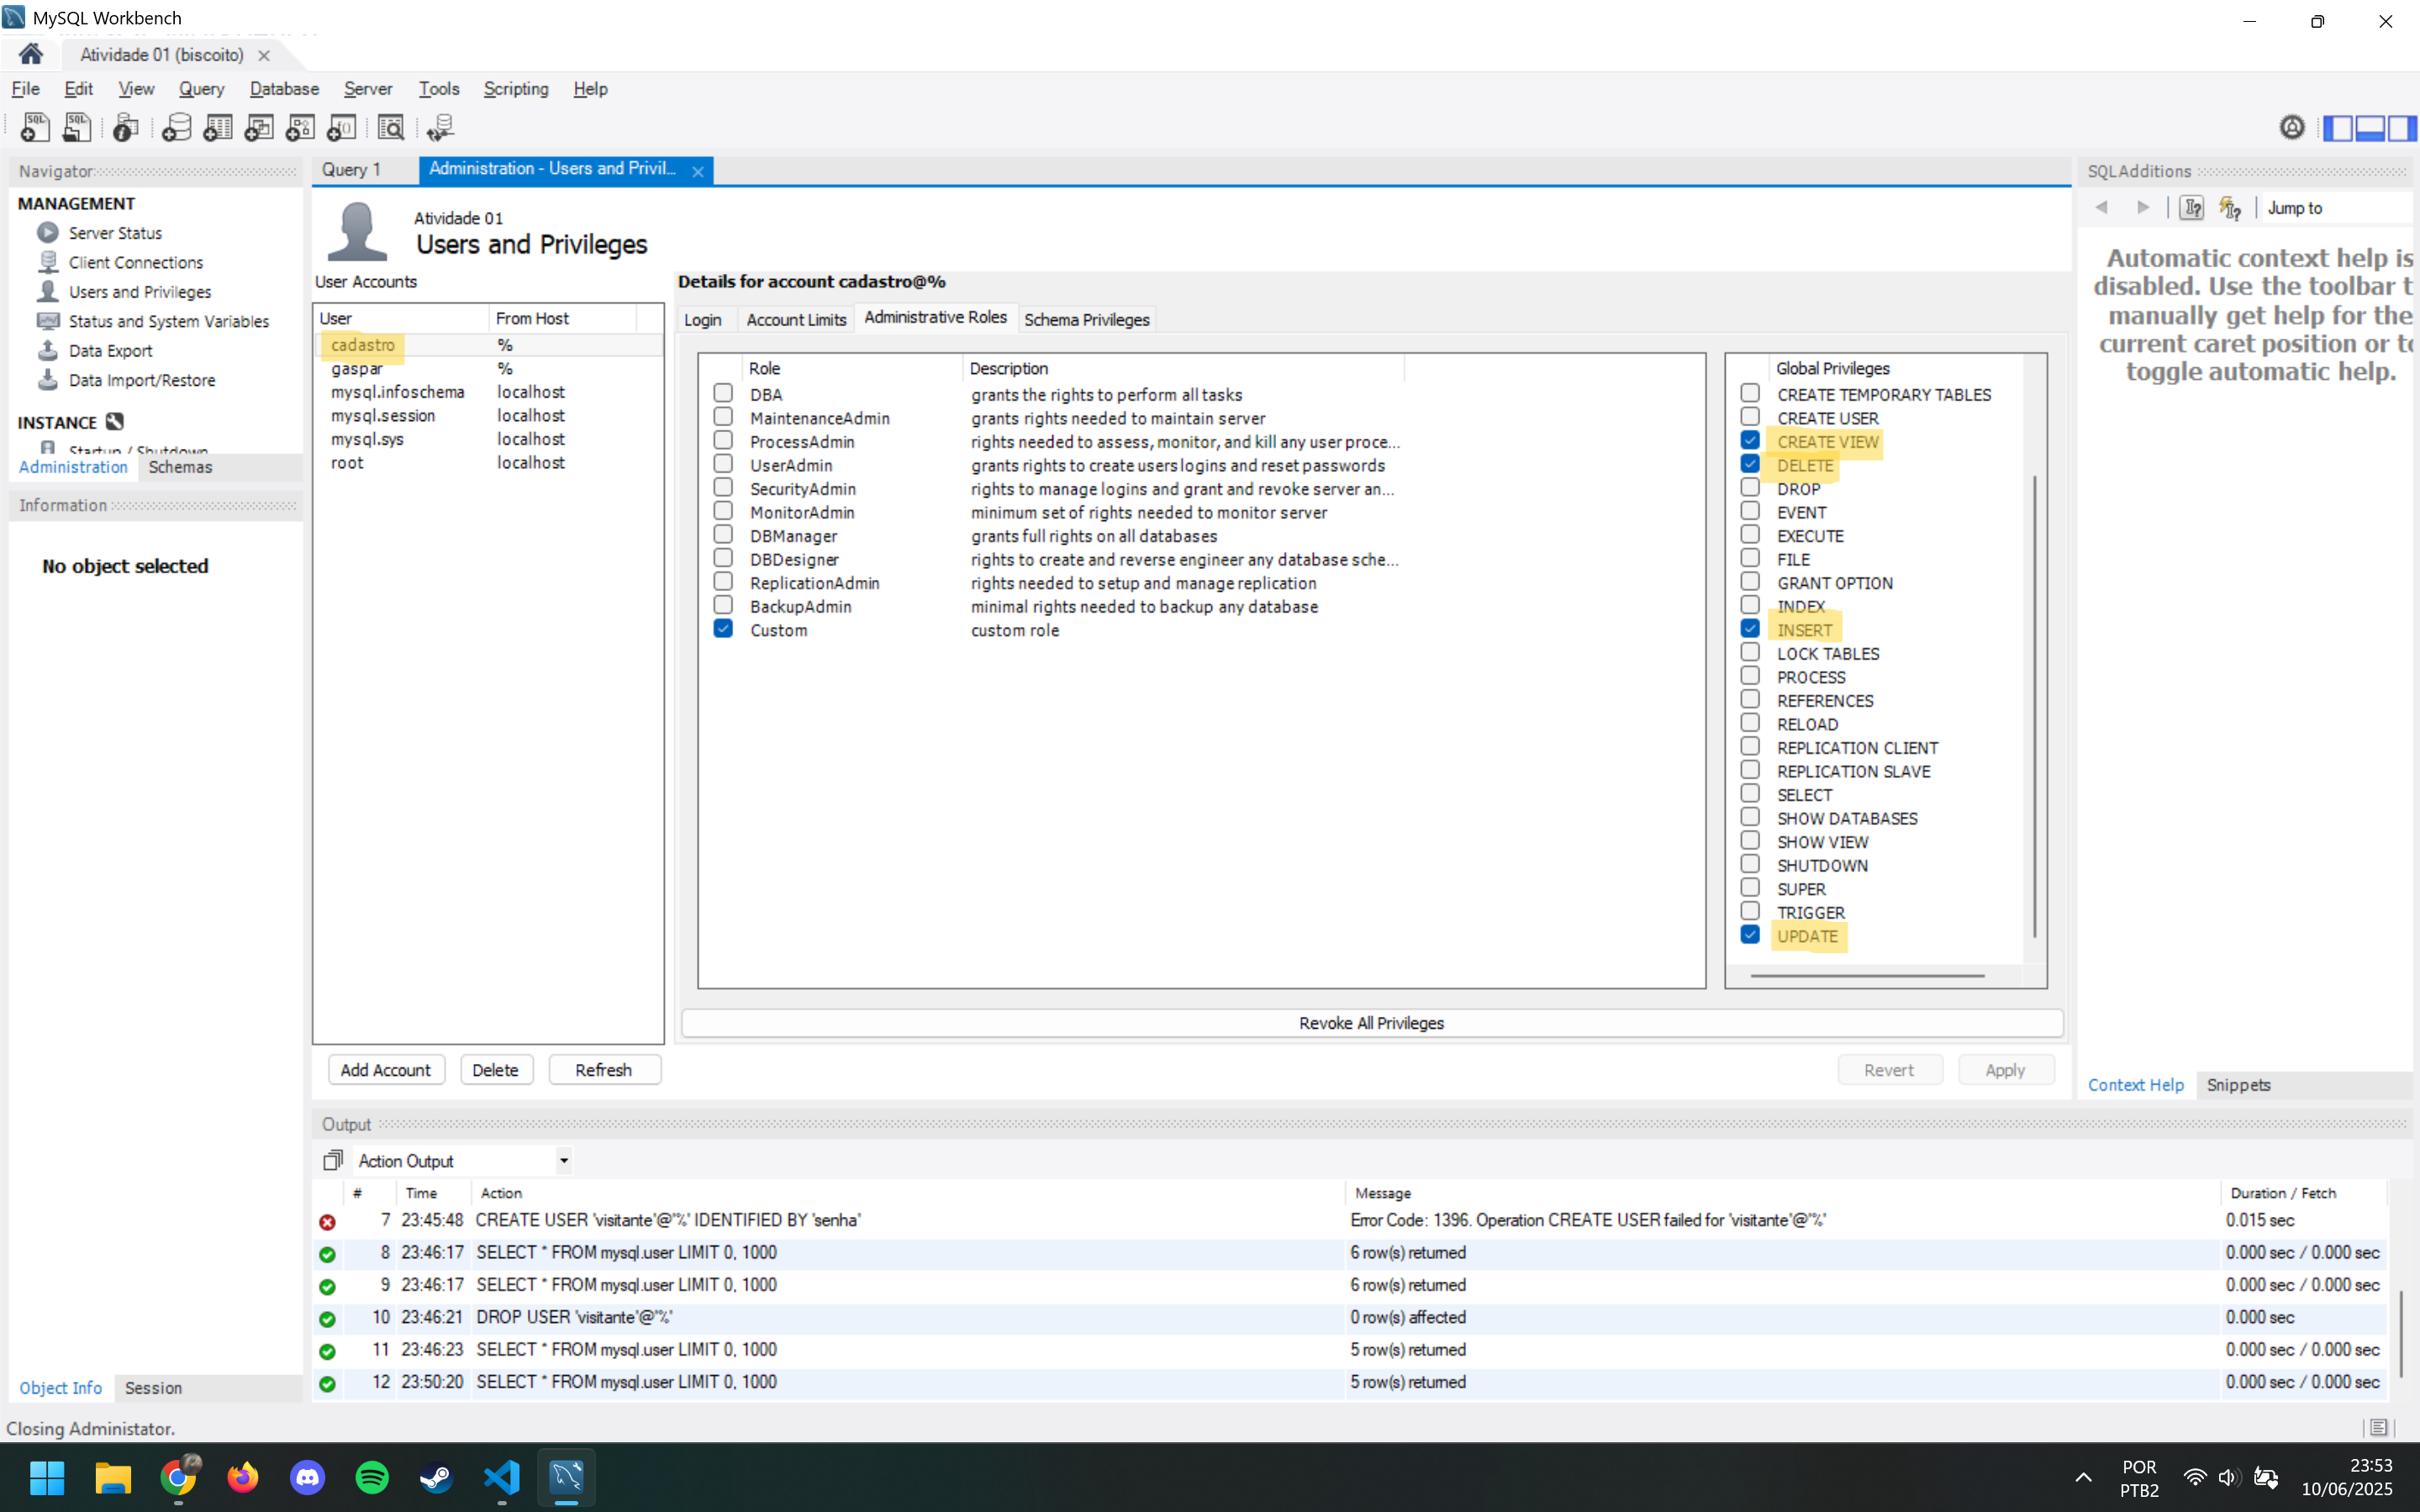
\includegraphics[width=0.95\linewidth]{g.png}
    \caption{Criação de usuário usando a GUI do MySQL}
    \label{fig:cadastroGUI}
\end{figure}

\section*{Exercício 5}
\paragraph{} Criando o novo banco de dados hipotético "pessoas", com o comando de forward engineer do MySQL:

\begin{lstlisting}[language=SQL]
    -- MySQL Workbench Forward Engineering

    SET @OLD_UNIQUE_CHECKS=@@UNIQUE_CHECKS, UNIQUE_CHECKS=0;
    SET @OLD_FOREIGN_KEY_CHECKS=@@FOREIGN_KEY_CHECKS, FOREIGN_KEY_CHECKS=0;
    SET @OLD_SQL_MODE=@@SQL_MODE, SQL_MODE='ONLY_FULL_GROUP_BY,STRICT_TRANS_TABLES,NO_ZERO_IN_DATE,NO_ZERO_DATE,ERROR_FOR_DIVISION_BY_ZERO,NO_ENGINE_SUBSTITUTION';

    -- -----------------------------------------------------
    -- Schema pessoas
    -- -----------------------------------------------------

    -- -----------------------------------------------------
    -- Schema pessoas
    -- -----------------------------------------------------
    CREATE SCHEMA IF NOT EXISTS `pessoas` DEFAULT CHARACTER SET utf8 ;
    USE `pessoas` ;

    -- -----------------------------------------------------
    -- Table `pessoas`.`pessoa`
    -- -----------------------------------------------------
    CREATE TABLE IF NOT EXISTS `pessoas`.`pessoa` (
    `cpf` VARCHAR(14) NOT NULL,
    `nome` VARCHAR(100) NOT NULL,
    `sexo` CHAR(1) NOT NULL,
    `nascimento` DATE NOT NULL,
    PRIMARY KEY (`cpf`))
    ENGINE = InnoDB;


    SET SQL_MODE=@OLD_SQL_MODE;
    SET FOREIGN_KEY_CHECKS=@OLD_FOREIGN_KEY_CHECKS;
    SET UNIQUE_CHECKS=@OLD_UNIQUE_CHECKS;
\end{lstlisting}

\paragraph{} Para criar o usuário "fazNada" e atribuir as permissões:

\begin{lstlisting}[language=SQL]
    CREATE USER 'fazNada'@'%' IDENTIFIED BY 'senha';
    GRANT INSERT(cpf) ON pessoas.pessoa TO 'fazNada'@'%';
\end{lstlisting}

\paragraph{} Para o usuário inserir CPFs na tabela, se usaria a seguinte query:

\begin{lstlisting}[language=SQL]
    INSERT INTO pessoa (cpf) VALUES (12345678901);
\end{lstlisting}

\paragraph{} Mas, como a coluna de nome, sexo e nascimento estão vazias, não é possível inserir nada com o usuário "fazNada". Esse tipo de restrição, neste caso, é desnecessário e sem nexo, já que não é possível inserir um CPF sem um nome, sexo e data de nascimento na tabela pessoa. 

\section*{Exercício 6}

\begin{enumerate}[label=\alph*)]
    % letra A
    \item Não. Em caso de vazamentos, todas as senhas que foram vazadas, não tem nenhum tipo de proteção.
    
    % letra B
    \item Poderia ser utilizado um método de criptografia unidirecional, como SHA2, que você só pode encriptar, mas não descriptografar (por isso o nome unidirecional).
    
    % letra C
    \item A função MD5, é um tipo de hash, no qual é feito com uma string de qualquer tamanho e codificando ela em uma impressão digital de 128 bits. Codificando a mesma string, sempre retornará o mesmo hash de 128 bits. A função MD5 é amplamente utilizada ao salvar senhas, números de cartão de crédito e outros tipos de dados sensíveis em banco de dados, como o MySQL. Além de criptografia, a função MD5 também é utilizada para garantir integridade de arquivos, considerando que uma string sempre retornará uma hash de 128 bits, o usuário pode comparar o hash do arquivo fonte com um hash recém criado do arquivo de destino, garantindo que o arquivo original não foi adulterado.
    
    % letra D
    \item Feita pela NSA (Agência de Segurança Nacional dos EUA), SHA1 (Secure Hash Algorithm 1), é uma função hash que converte os dados de entrada em um valor de hash de 160 bits, normalmente exibido como um valor hexadecimal de 40 caracteres. Assim como a função MD5, é uma função unidirecional, então, tendo somente a hash resultante, é praticamente impossível descriptografar a mesma. A sua função também é igual a da MD5. As suas diferenças estão na hash resultante, que a função MD5 retorna uma hash de 128 bits, enquanto a SHA1 retorna uma de 160 bits.
    
    % letra E
    \item Assim como seu precursor, SHA1, feito pela NSA, o SHA2 serve praticamente o mesmo propósito do SHA1, com a principal diferença sendo que ela é composta por seis funções diferentes, com valores que são de 224, 256, 384 ou 512 bits, sendo elas a SHA-224, SHA-256, SHA-384, SHA-512, SHA-512/224, SHA-512/256.
    \par Para usar essa função no MySQL, é utilizado a seguinte query, com o primeiro argumento sendo o texto simples e o segundo sendo o tamanho de bits desejado do resultado. Por exemplo:
    
    \begin{lstlisting}[language=SQL]
        SELECT SHA2('textosimples', 256) AS SHA2;
        -> '1d400a2a67d36062aa4006d2ce28b20545bb25ccf2dcea78ba98e94389de7dfb'
    \end{lstlisting}

    % letra F
    \item A função AES\_ENCRYPT é usada para criptografar dados usando o algoritmo AES (Advanced Encryption Standard). Ela recebe um valor e uma chave como parâmetros e retorna os dados criptografados. Para visualizar ou armazenar o resultado, é comum converter para hexadecimal ou base 64, caso contrário o resultado criptografado será um blob. Por exemplo:

    \begin{lstlisting}[language=SQL]
        SELECT TO_BASE64(AES_ENCRYPT('texto', 'chave'));
        -> 'm80MMJKdDw9nSHlUXyEPYA=='
    \end{lstlisting}

    \par Para descriptografar, e para que o texto de saída não seja um blob, se usa a seguinte query:

    \begin{lstlisting}[language=SQL]
        SELECT CAST(AES_DECRYPT(FROM_BASE64('m80MMJKdDw9nSHlUXyEPYA=='), 'chave') AS CHAR);
        -> 'texto'
    \end{lstlisting}

    % letra G
    \item É praticamente impossível descriptografar a senha dada, já que ela está de acordo com a saída de um MD5. Como o MD5 é unidirecional, não tem alguma maneira viável de fazer isso.
    
    % letra H
    \item Mesma coisa do item acima, é praticamente impossível descriptografar a senha dada, já que ela está de acordo com a saída de um SHA1. Como o SHA1 é unidirecional, não tem alguma maneira viável de fazer isso.
    
    % letra I
    \item Foi criado uma coluna \textit{senha char(64) NOT NULL}, para armazenar senhas de acordo com o SHA2-256
    \begin{lstlisting}[language=SQL]
        ALTER TABLE pessoa ADD COLUMN senha CHAR(64) NOT NULL;
    \end{lstlisting}
    
    % letra J
    \item Para inserir um registro, utilizando a função SHA2-256() para senha:

    \begin{lstlisting}[language=SQL]
        INSERT INTO pessoa VALUES (12345678901, 'Eduardo Tieppo', 'M', '1988-11-23', SHA2('senha', 256));
    \end{lstlisting}

    % letra K
    \item Usando a query dada e trocando o nome da coluna e a senha, retorna corretamente:

    \begin{lstlisting}[language=SQL]
        SELECT * FROM pessoa WHERE senha = SHA2('senha',256);
        -> '12345678901', 'Eduardo Tieppo', 'M', '1988-11-23', 'b7e94be513e96e8c45cd23d162275e5a12ebde9100a425c4ebcdd7fa4dcd897c'
    \end{lstlisting}

    % letra L
    \item Considerando os exercícios anteriores desta lista, é possível chegar a conclusão que o método mais seguro de se guardar uma senha é usando a função SHA2-512, com restrições no tamanho e caracteres disponíveis para usar na senha. Por exemplo, se a senha tiver o mínimo de 8 caracteres e o máximo de 16 caracteres, com somente letras minúsculas e maiúsculas, sem acentuação, números de 0 a 9 e pontuação básica, sendo elas \texttt{! @ \# \$ \% \& * ( )}. Considerando todas essas restrições, a chance de ter duas ou mais strings diferentes, nas quais resultem no mesmo hash, é tão próximo de zero, podendo até se afirmar que é impossível de existir senhas que tenham o mesmo hash. Por fim, isso torna impossível, sem bruteforce, descobrir uma senha que esteja salva em SHA2. 

\end{enumerate}


\end{document}